\chapter{Introduction}
Today software applications in some form or another is used in every aspect of our lives. Softwares are being constantly developed to handle more complex issues while being scalable to millions of users and due to this complexity involved in development they may suffer from serious software implications such as exploitable malwares \& vulnerabilities. The study by Cui et al. showed that 80.4\% of vendor-issued firmware is released with multiple known vulnerabilities, and many recently released firmware updates contain vulnerabilities in third-party libraries that have been known for over eight years \cite{Cui}. 

Most malware's developed today are not created from scratch but in some way they are modification of some existing malware to create new ones. This can be used to our advantage by using code reuse detection to generate feature vectors for those and use with machine learning algorithms that can recognize new or similar malware or vulnerabilities \cite{Jang}. One of the other reason for analyzing binaries for finding vulnerabilities and plagiarism are often lack of source code because of third-party software \cite{Saeb} or not having access of source codes we wish to perform analysis on but almost everyone having access to binary (i.e., executable) code. Binary analysis is thus important for understanding the inner workings of malware or exploring vulnerabilities in existing systems but doing it manually is a very intensive task. Due of these challenges binary analysis is an very important area of research in computer science and automated tools which can do the analysis efficiently and effectively are in very high demand.

\section{Background}

Recently, there has been bloom in research to tackle the problem of binary code similarity detection. In binary code analysis detecting similar functions in binary executables remains one of the fundamental problem and is well known as ``binary code similarity detection'' problem. These efforts commonly involves extracting binary code into representable form either a vector or graph to represent functions of binary.  Then, it is checked that whether among extracted control flow graph functions representations any functions are similar or not using a graph matching algorithm.  

%since we are generally missing abstractions provided by programming languages making 
%binary analysis difficult \cite{Teresa} but there are some advantages 

Graph-based matching approaches have some drawbacks. One of them is their adaptability for different applications since they are approximated by fixed graph matching algorithm. For example, even the same code compiled with different optimization level may result in producing different control flow graphs since it will be not be matched by fixed graph matching\cite{Xu}. Other problem is due to inefficiency of graph matching algorithm (such as bipartite graph mathcing) which are considerably slow thus it will degrade the overall efficiency of code similarity detection since it heavily rely on the graph matching algorithm.  

A practical and efficient clone searching algorithm relies on a robust vector representation of assembly code. However, existing clone search approaches, rely on a manual feature engineering for every assembly function process to create its vector representation,which fail to identify unique patterns that can statistically distinguish assembly functions. However, it is a challenging problem to automatically pick the best representation of a function due to the fact that there are varieties of compiler optimizations and code obfuscation techniques that make equivalent assembly functions appear to be very different. These techniques have a strong impact on the resulting assembly instructions and the linear layout of the assembly code. Figure 1.1 shows some examples of assembly functions that correspond to the same source code. The major challenge is how to identify these semantically equivalent but structurally different assembly functions as clones.


\begin{figure}
	\centering
	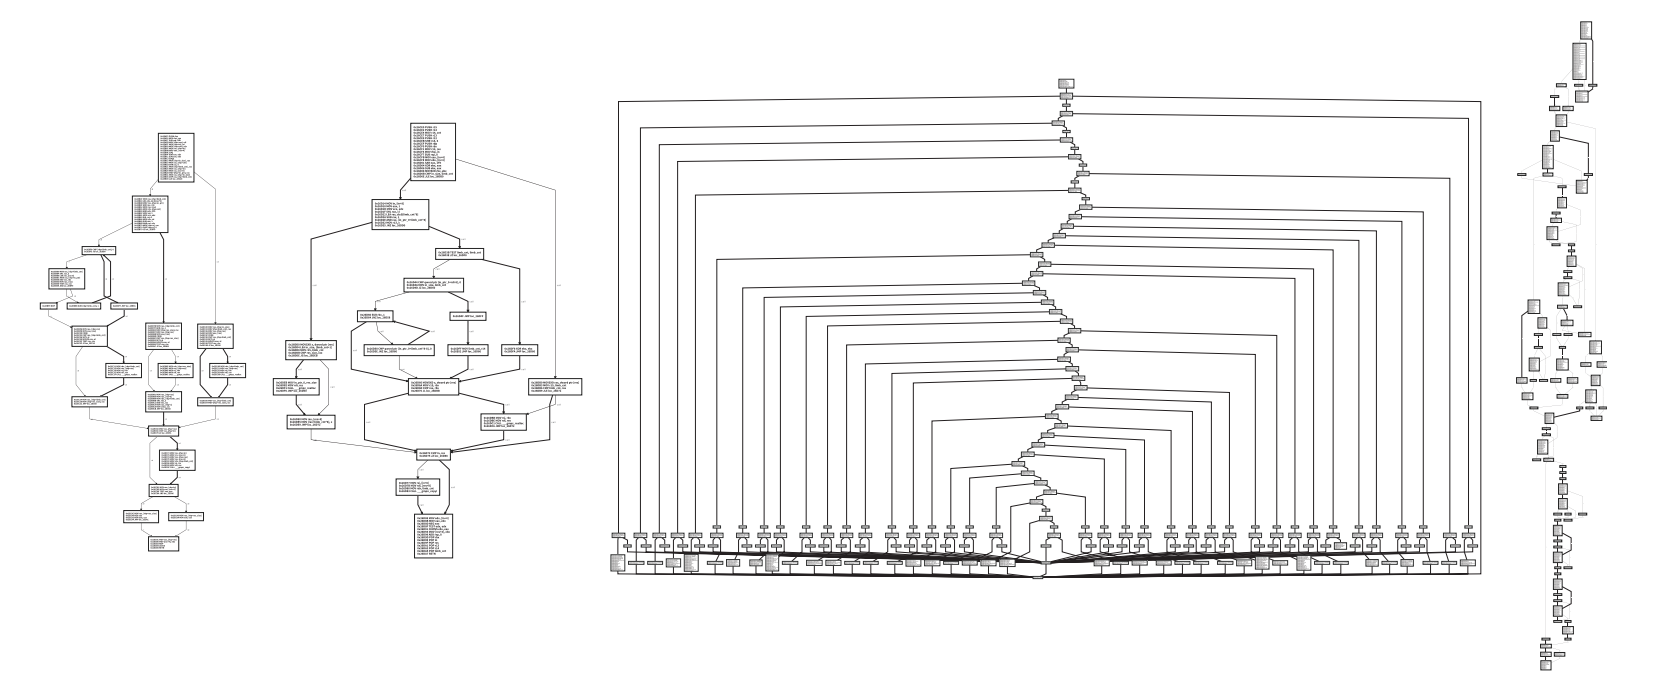
\epsfig{file=diff_cfgs.png, height=2.75in, width=6.5in}
	\caption{Different assembly functions compiled from the same \textit{gmpz\_tdiv\_r\_2exp} function of \textit{Libgmp}. From left to right, the assembly functions are compiled with the \textit{GCC O0} option, \textit{GCC O3} option, \textit{Obfuscator-LLVM} Control Flow Graph Flattening option and Bogus Control Flow Graph option.}
\end{figure}


Typically, the following four categories of features are used in the literature for assembly clone search.

\textbf{Token-based features :} These features model the similarity between two assembly code functions based on a set of tokens. The tokens can include constants, assembly instructions such as n-grams or n-perms \cite{Khoo}, or assembly instructions with normalized operands
\cite{Ding, Farhadi, Andreas}. Typically, the frequency value is used to construct the feature vector. Constant tokens are robust if they are weighted correctly. Some common constants such as the ones used for stack manipulation are insufficient to distinguish assembly functions, which leads to a relatively lower level of recall rate as shown in \cite{Khoo}. Instruction-based tokens have a weak robustness since the selected compiler, compiler optimization settings, and the obfuscation techniques all have a strong influence on the choice of instructions. The same logic can be expressed differently in assembly code. More importantly, instruction tokens used as features fail to capture the semantic relationship between tokens. For example, the assembly instructions Add and Sub are similar in the sense that they are both arithmetic instructions. To address this problem, in [7, 9] instructions are classified into categories such as transfer, algorithmic, and stack operations, among others. However, they fail to model the relationship between instructions across different categories. The best way is to learn the relationship directly from data. Let the assembly code itself show what assembly instructions are similar by considering the context in which they co-occur. For example, instructions appearing around stack registers are similar as they somehow relate to stack manipulation. Likewise, instructions appearing around floating point registers are similar in the sense that they somehow relate to floating point operations and vice versa.

\textbf{Text-based features :} Studies such as \cite{David} fall into this category. It models the similarity between two assembly functions or frag- ments based on a customized string editing distance. String editing distance is not robust, since the linear layout of the assembly code
can be modified  easily. Obfuscator can substitute instructions with their semantically equivalent but syntactically different form, which leads to a very different editing distance. A good representation of assembly code should be able to identify position-invariant patterns
that is robust to different linear layouts.

\textbf{Graph-based features :} Studies under this category compare assembly functions using subgraph isomorphism algorithms \cite{Ding, Eschweiler, Pewny} or a set of graph substructures \cite{Feng, Khoo, Kruegel} as features. Graph-based features rely on the correct detection of basic block boundaries
and reconstruction of Control Flow Graphs (CFG). Graph-based features are not robust, since different compiler optimization settings can already significantly change the control flow graph by loop unrolling and function inlining. Some approaches use subgraphs that consists of 2-3 nodes as features \cite{Khoo, Kruegel}. Their robustness is therefore enhanced. Even if the CFG is heavily modified, some important logics and subgraph structures still remain the same.
These features are less sensitive to CFG modifications. However, a graph flattening obfuscation technique from Obfuscator-LLVM (O-LLVM) \cite{Junod} that destroys all the subgraph structures can make
the graph-based features useless.

\textbf{Dynamic features :} Studies under this category dynamically execute fragments of assembly code and use them as features \cite{Chandramohan, David, Pewny}. These features normalize assembly instructions that are semantically equivalent but syntactically different. However, one of the main problems is that it requires a pair-wise full permutation of  input/output variables to match the symbolic expressions extracted from the assembly code. This process is slow and can hardly be scalable without developing a specialized indexing schema for symbolic expression. Moreover, different assembly instructions have different side effects such as setting the flag bits. When matching assembly functions, it is difficult to determine what is the main logic and what would be the correct set of input and output. 


All the aforementioned approaches are based on the manual feature engineering process, several assumptions are made. Thus, the chosen representation may not truly embrace the important patterns that distinguish one assembly function from another. Deep learning \cite{LeCun} in recent years has be involved in many application domains which also includes binary analysis and has concluded pretty interesting results than other approaches. Deep learning allow us to learn representations of data(vector or graphical) with multiple levels of abstraction freeing involvement of any domain knowledge which is very big advantage of using it. It is also very adaptive and can be modified to train on data of our particular interest and can be utilized in our approach.

\section{Purpose}

We propose a novel approach, for assembly clone detection. It is different from graph-based methods since we first extracts the information from the binaries and feed this information to Neural Network to generate an embedding (vector representation) of the functions. All previous research on assembly code clone relies on the manual feature engineering process. Our vector representation of assembly code as a way to mitigate the afore mentioned issues in current handcrafted features. Combining the graph embedding networks into a Siamese network \cite{Bromley} naturally captures the objective that the graph embeddings of two similar functions should be close to each other and vice versa. This entire network model can then be trained end-to-end for similarity detection. Further, we design a new training and dataset creation method using a default policy to pre-train a task-independent graph embedding network. The learning process does not also require any prior knowledge about assembly code, such as compiler optimization settings or the correct mapping between assembly functions. It only needs assembly code functions. We discuss the differences between the assembly code and text data, as well as the issues we had in applying the representation learning on assembly code.

Our approach constructs a large-scale training dataset using binary functions compiled from the same source code but for different platforms and compiler optimization levels. Our evaluation demonstrates that this task-independent model is more effective and generalize better to unseen functions than the state-of-the-art graph matching-based approach \cite{Dullien}. One advantage of the neural network-based approach is that the pre-trained model can be retrained quickly in the presence of additional supervision to adapt to new application scenarios. Our evaluation shows that with such additional supervision, the retrained model can efficiently adapt to novel tasks. This efficiency property enables practical usage of the retraining to improve the quality of similarity detection. We have implemented a prototype called Gemini. In a broader scope, this work showcases a successful example of how to apply deep learning to solve important and emerging computer security problems and substantially improves over the
state-of-the-art results. We conduct extensive experiments with all the combinations of optimization levels in the GNU GCC compiler. We benchmark various state-of-the-art assembly clone search techniques in the experiment. We show that by using representation learning, a simple cosine-similarity-based approach significantly outperforms the others regarding both recall and precision.

%and different obfuscation techniques of Obfuscator-LLVM [14] with the CLANG compiler. It is the first clone search experiment that covers a strong obfuscator which substitutes instructions, splits basic blocks, adds bogus logics, and completely destroys the original control flow graph.
 

\section{Outline}
We summarize our contributions as follows:

\begin{itemize}
	\item We propose the neural network-based approach to generating embeddings for binary functions.
	\item We propose a novel approach to train the embedding network using a Siamese network so that a pre-trained model can generate embedding to be used for similarity detection.
	\item We propose a retraining approach so that the pre-trained 	model can take additional supervision to adapt to specific tasks.
	\item We implement a prototype and our evaluation demonstrates that on a test set constructed from OpenSSL, it can achieve a higher AUC than previous state-of-the-art graph matching-based approach;
\end{itemize}


The rest of the thesis is organized as follows. Chapter 2 gives detailed introductions to several different topics that is used throughout the thesis. Chapter 3 contains describes the approach and an overview of implementation used for the binaries analysis required by this project. Chapter 4 presents results obtained during the evaluation of the system developed Finally, Chapter 5 presents conclusions regarding binary analysis based code similarity detection of with suggestions for future work.
